% !TeX root = ../../../main.tex

The aim of this  section is to scrutinize the \pdf dependence of the
neutral-current \acrlong{dy} differential cross-section and of the associated
forward-backward asymmetry by reviewing the \lo kinematics, determining \lo
analytic expressions, and finally comparing these analytical calculations to
the results of \lo and \nlo  numerical simulations obtained using \mgamc,
\cite{Alwall:2014hca}, interfaced to \pineappl,
\cite{Carrazza:2020gss,christopher_schwan_2022_7023438}.
%
Specifically, we will relate the behavior of the differential distribution and
asymmetry to the relevant parton luminosities.

\subsection{Drell-Yan kinematics and cross-sections at \lo}
\label{sec:dylo}

We consider dilepton production via the exchange of an electroweak neutral
gauge boson $Z/\gamma^*$ in proton-proton collisions:
\begin{equation}
  \label{eq:DYprocess}
  \mathrm{p}(k_1) + \mathrm{p}(k_2) \to Z/\gamma^*(q) \to \ell(p_{\ell}) + \bar{\ell}(p_{\bar{\ell}}) + X \text{.}
\end{equation}
The hadronic differential cross-section $\dd\sigma^{\mathrm{p}\mathrm{p}\to\llb}$  is factorized in
terms of \pdfs $f_i$ and the partonic cross sections
$\dd\hat\sigma_{ij}$ for incoming partons of species $i,\,j$ as
\begin{equation}
  \dd\sigma^{\mathrm{p}\mathrm{p}\to\llb} = \sum_{ij} \int\limits_0^1\!\dd x_1 \dd
  x_2 f_i(x_1,\mu_F^2) f_j(x_2,\mu_F^2) \dd\hat\sigma_{ij}(\hat k_1 = x_1
  k_1, \hat k_2 = x_2 k_2).
  \label{eq:factorization}
\end{equation}
In the sequel we will set the  factorization scale $\mu_F$ to the
invariant mass of the gauge boson, i.e.\ the dilepton
invariant mass, so $\mu^2_F = \mll^2=(p_\ell + p_{\bar{\ell}})^2$.
%
The kinematics and Feynman diagram of the \lo partonic process
in the quark-antiquark channel are shown in \cref{fig:lo-dy}.
We do not consider photon-initiated processes, as they do not affect
the qualitative features of our discussion.

%--------------------------------------
\begin{figure}[t]
  \centering

  \begin{tikzpicture}
    \begin{feynman}
      \tikzfeynmanset{large}

      \vertex (b);
      \vertex [above left=of b] (a) {\(q\)};
      \vertex [below left=of b] (f1) {\(\bar{q}\)};
      \vertex [right=of b] (c);
      \vertex [above right=of c] (f2) {\(\ell\)};
      \vertex [below right=of c] (f3) {\(\bar{\ell}\)};

      \diagram* {
      (a) -- [fermion, momentum=\(\hat{k}_1\)] (b) -- [fermion, rmomentum=\(\hat{k}_2\)] (f1),
      (b) -- [boson, edge label'=\(\gamma / Z\), momentum=\(q\)] (c),
      (c) -- [anti fermion, momentum=\(p_{\ell}\)] (f2),
      (c) -- [fermion, momentum=\(p_{\bar{\ell}}\)] (f3),
      };
    \end{feynman}
  \end{tikzpicture}

  \caption{Neutral-current Drell-Yan production at \lo in the quark-antiquark channel.}
  \label{fig:afb/lo-dy}
\end{figure}

%--------------------------------------

At \lo, the momentum fractions of the two incoming partons are fully
fixed by knowledge of the invariant mass and rapidity of the gauge
boson, i.e.\ of the dilepton pair  $\yll = (y_\ell + y_{\bar{\ell}})/2$: 
\begin{equation}
  \label{eq:x_fractions}
  x_1 = \frac{ \mll}{\sqrt{s}}\exp(\yll) \, ,\quad x_2 = \frac{
  \mll}{\sqrt{s}}\exp(-\yll) \, ,
\end{equation}
where the center of mass energy of the hadronic collision is
$s=(k_1+k_2)^2$ and at \lo
$\mll^2 = \hat s = x_1 x_2 s$. The absolute dilepton
rapidity thus lies in the range $|\yll|\le \ln (\sqrt{s}/\mll)$.
Beyond \lo there might be extra radiation in the final state, so the \lo
kinematics provides a lower bound on the momentum fractions of the
incoming partons, and all values of the momentum
fractions such that $x_{1,2}\ge \mll/\sqrt s$ are allowed.

It is useful to define the so-called  Collins-Soper
angle $\theta^*$~\cite{Collins:1977iv}, which in the hadronic \acrfull{com}
frame is defined as
\begin{equation}
\begin{split}
  \cos\theta^* &= \sign (\yll) \cos\theta \, ,\\
  \cos\theta &\equiv\frac{p_\ell^+ p_{\bar{\ell}}^- - p_\ell^- p_{\bar{\ell}}^+}{\mll \sqrt{\mll^2 + p_{\mathrm{T},\ell\bar{\ell}}^2}} \text{,} \quad p^\pm = p^0 \pm p^3 \text{.}
  \label{eq:cosine-cs-angle}
\end{split}
\end{equation}
It is easy to show that the Collins-Soper angle $\theta^*$ coincides with the
scattering angle of the lepton in the partonic \com frame, $\bar\theta$.
%
The latter is defined in terms of the lepton momentum as 
\begin{equation}
 \cos\bar\theta \equiv \frac{p^z_\ell}{\mll} \,, \label{eq:coscm}
\end{equation}
where the $z$ axis is along the direction of the incoming quark-antiquark pair.
%
In the partonic \com frame, of course, $p^z_\ell=-p^z_{\bar \ell}$ and $\yll
=0$, so
\begin{equation}
p^\pm_\ell=p^{\mp}_{\bar{\ell}}=  \mll \left( 1\pm \cos{\bar\theta} \right)\, ,
\end{equation}
and substituting in \cref{eq:cosine-cs-angle} it immediately follows that,
taking the convention 
$\sign (\yll)=\sign(0)=+1$, 
$\cos\theta^*=\cos\theta=\cos{\bar\theta}$.
%
The expression of $\cos\theta$ in \cref{eq:cosine-cs-angle} is manifestly
invariant upon boosts along the $z$ axis, so the identification of $\theta$
with the \com scattering angle $\bar\theta$ remains true in any reference
frame.

Note that the definition \cref{eq:coscm} requires a choice for the positive
direction of the $z$ axis, which is usually taken along the direction of the
incoming fermion (quark).
%
This direction is  not experimentally accessible in proton-proton collisions,
so the Collins-Soper angle is defined by always taking the positive $z$ axis in
the direction of the boosted dilepton pair, i.e., at \lo, along the direction of
the incoming quark with largest momentum fraction, i.e.\ by supplementing in
the definition a factor $\sign(\yll)$.
%
Hence $\cos\theta^*=\cos{\bar\theta}$ ($\cos\theta^*=-\cos{\bar\theta}$)  if
the momentum fraction of the incoming quark (antiquark) is the largest.

%
The hard scattering matrix elements that enter the partonic cross-section
in \cref{eq:factorization} are the sum of a pure photon-exchange
contribution, a photon-$Z$ interference term, and a pure $Z$-exchange
contribution.
%
Of course, in the region
$\mll \gtrsim m_Z$ these contributions are all of the same order.
%
Standard arguments~\cite{Peskin:1995ev} then imply that, because in the
Standard Model the photon
coupling to leptons is vector  while the $Z$ coupling is chiral,
the pure photon and pure $Z$ contributions to the cross-section are
necessarily  even in $\cos\theta^*$ while the interference term is
odd.

Specifically, at \lo the fully differential hadronic cross-section can
be obtained from the well-known result~\cite{Peskin:1995ev} for
$e^+e^-\to\mu^+\mu^-$ by replacing the incoming lepton charges  with
those of the quarks, and accounting for the \pdfs, with
the result
\begin{align}
    \frac{\dd^3 \sigma}{\dd \mll \, \dd \yll \, \dd\cos\theta^*} &= \frac{\pi \alpha^2}{3 \mll s} \left((1+\cos^2({\theta^*})) \sum_q S_q \left[f_q(x_1,\mll^2) f_{\bar{q}}(x_2,\mll^2) + f_q(x_2,\mll^2) f_{\bar{q}}(x_1,\mll^2) \right] \right. \nonumber\\
    &\hspace*{15pt} + \left. \cos\theta^* \sum_q A_q \sign (\yll) \left[ f_q(x_1,\mll^2) f_{\bar{q}}(x_2,\mll^2) - f_q(x_2,\mll^2) f_{\bar{q}}(x_1,\mll^2)\right] \right) \, ,
    \label{eq:lo-triple-diff}
\end{align}
where  $\alpha$ is the QED coupling and the even (symmetric) and
odd  (antisymmetric) couplings are given by
\begin{align}
  \label{eq:coup}
    S_q &= e_l^2 e_q^2 + P_{\gamma Z} \cdot  e_l v_l e_q v_q + P_{ZZ} \cdot  (v_l^2+a_l^2)(v_q^2+a_q^2) \nonumber \\
    A_q &= P_{\gamma Z} \cdot 2 e_l a_l e_q a_q  + P_{ZZ} \cdot 8 v_l a_l  v_q a_q \, ,
\end{align}
in terms of the electric charges  $e_l$, $e_q$ and the vector and
axial couplings $v_l$, $v_q$ and $a_l$, $a_q$  of the leptons and
quarks, and the propagator factors
\begin{align}\label{eq:propgz}
    P_{\gamma Z}(\mll) &= \frac{2\mll^2 (\mll^2  - m_Z^2)}{\sin^2(\theta_W) \cos^2(\theta_W)\left[(\mll^2 - m_Z^2)^2 + \Gamma_Z^2 m_Z^2\right]}\\
\label{eq:propzz}
    P_{ZZ}(\mll) &= \frac{\mll^4}{\sin^4(\theta_W) \cos^4(\theta_W)\left[(\mll^2 - m_Z^2)^2 + \Gamma_Z^2 m_Z^2\right]},
\end{align}
with $m_Z$  and $\Gamma_Z$ respectively the $Z$ mass and width and $\theta_W$ the weak mixing angle.
%
In \cref{fig:lo-couplings} we display the
symmetric $S_q$ (left) and antisymmetric $A_q$ (right)
couplings, \cref{eq:coup}, for up-like and
down-like quarks, as a function of 
the dilepton invariant mass $\mll$.
%
Both couplings are around a factor 2 larger for
up-like quarks than for down-like quarks, and
become $\mll$-independent for $\mll \gsim 1$ TeV, where they take
the asymptotic values $\bar S_q$, $\bar A_q$ obtained by
substituting in \cref{eq:coup} the large-mass expressions of
the propagator factors
\begin{equation}\label{eq:propasympt}
    \bar P_{\gamma Z} = \frac{2}{\sin^2(\theta_W)\cos^2(\theta_W)},
    \qquad 
    \bar P_{ZZ} = \frac{1}{\sin^4(\theta_W) \cos^4(\theta_W)},
\end{equation}
to which $P_{\gamma Z}$ and $P_{ZZ}$ respectively reduce up to $O(m^2_Z/\mll^2)$ corrections.

 
%%%%%%%%%%%%%%%%%%%%%%%%%%%%%%%%%%%%%%%%%%%%%%%%%%%%
\begin{figure}
  \centering
  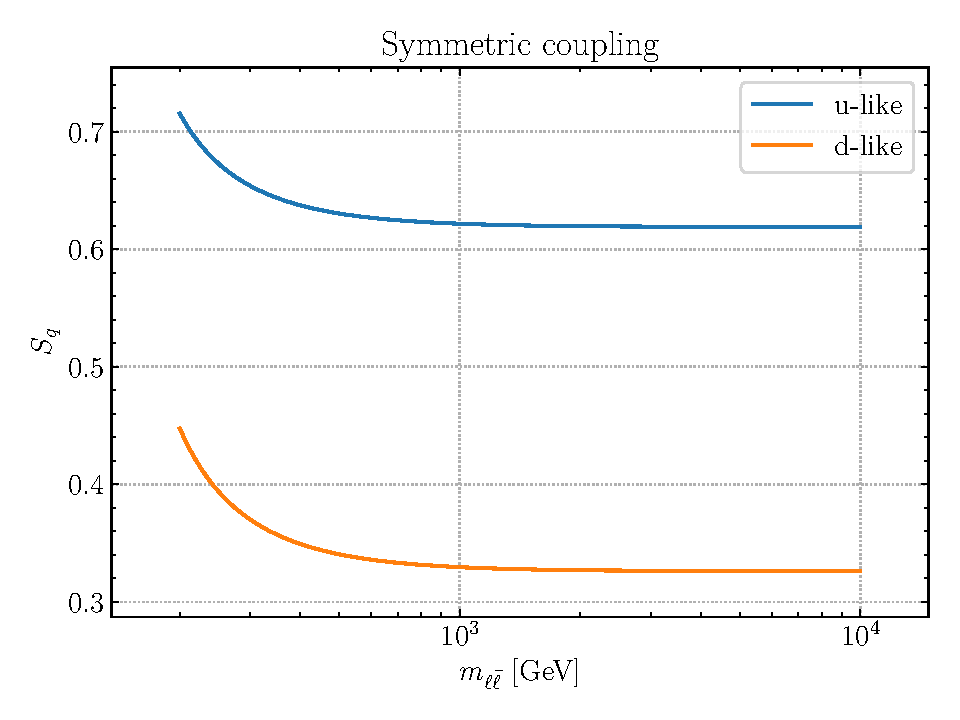
\includegraphics[width=0.49\linewidth]{ch-afb/symmetric-couplings.pdf}
  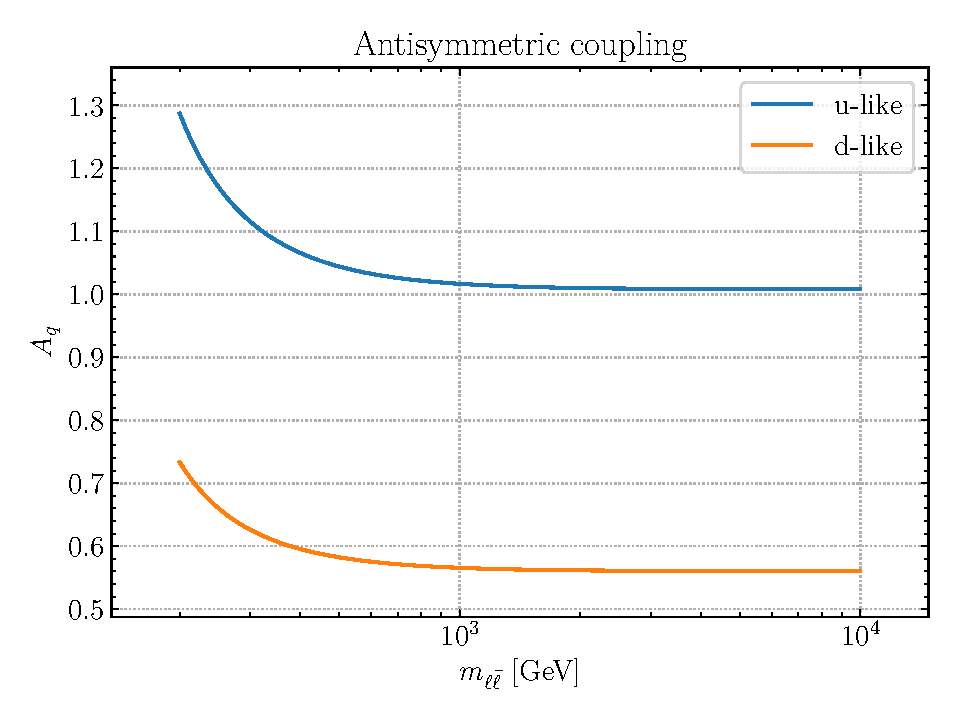
\includegraphics[width=0.49\linewidth]{ch-afb/antisymmetric-couplings.pdf}
  \caption{The symmetric $S_q$ (left) and antisymmetric $A_q$ (right)
    couplings, \cref{eq:coup}, for up-like and
    down-like quarks, as a function of 
 the dilepton invariant mass $\mll$.
  }
  \label{fig:lo-couplings}
\end{figure}
%%%%%%%%%%%%$$$$$$$$$$$$$$$$$$$$$%%%%%%%%%%%%%

The interference term proportional to
$A_q$ is odd in the Collins-Soper angle $\cos\theta^*$, leading to a forward-backward
scattering asymmetry.
%
In a proton-proton collision the initial state is completely
symmetric, so the quark and antiquark contributions to the
cross-section \cref{eq:lo-triple-diff} are necessarily symmetric
upon the interchange of the incoming quark and antiquark, with the
corresponding momentum fractions fixed at \lo by
\cref{eq:x_fractions}.
%
However, as mentioned, there
is a sign change in the relation between $\cos\theta^*$ and
$\cos\theta$ according to whether the incoming parton with largest
momentum fraction is a quark or an antiquark, i.e.,
when interchanging
$x_1$ with $x_2$ in the argument of the quark and antiquark \pdfs,
thereby leading to the result of  \cref{eq:lo-triple-diff}.
%
This leads
to a forward-backward asymmetry whenever the quark and antiquark
\pdfs have different $x$ dependence.

In order to understand the relation of this forward-backward
asymmetry in terms of the
behavior of the \pdfs, it is convenient
to rewrite the \pdf combinations that contribute to the differential
cross-section \cref{eq:lo-triple-diff} in terms of symmetric and
antisymmetric parton luminosities, defined as
\begin{align}
  \mathcal{L}_{S,q}(\mll, \yll) &\equiv f_q(x_1,\mll^2) f_{\bar{q}}(x_2,\mll^2) + f_q(x_2,\mll^2) f_{\bar{q}}(x_1,\mll^2) \, ,
  \nonumber\\
  \mathcal{L}_{A,q}(\mll, \yll) &\equiv \sign (\yll) \left[ f_q(x_1,\mll^2) f_{\bar{q}}(x_2,\mll^2) - f_q(x_2,\mll^2) f_{\bar{q}}(x_1,\mll^2)\right] \, , \label{eq:symm_asymm_lumis}
\end{align}
where the momentum fractions $x_1$ and $x_2$ are given in terms of $\mll$, $\yll$,
and $\sqrt{s}$ in \cref{eq:x_fractions}.
Note that both parton luminosities are invariant under
the interchange $x_1\leftrightarrow x_2$, upon which $\yll \to -\yll$.
%
In terms of these luminosities, the triple differential cross-section \cref{eq:lo-triple-diff}
takes the compact form
\begin{equation}
  \label{eq:lo-triple-diff-lumis}
  \frac{\dd^3 \sigma}{\dd \mll \, \dd \yll \, \dd\cos\theta^*} =
  \frac{\pi \alpha^2}{3 \mll s} \left( (1+\cos^2({\theta^*})) \sum_q S_q \mathcal{L}_{S,q}(\mll, \yll)
  + \cos\theta^* \sum_q A_q \mathcal{L}_{A,q}(\mll, \yll)  \right) \, ,
\end{equation}
which explicitly displays
its symmetry properties upon the transformation $\cos\theta^* \to -\cos\theta^*$,
equivalent to a charge conjugation transformation 
$q\leftrightarrow \bar q$ and $\ell \leftrightarrow \bar{\ell} $.

The symmetric and antisymmetric parton luminosities \cref{eq:symm_asymm_lumis} can also be expressed
in terms of the sum and difference of quark and antiquark \pdfs,
\begin{equation}
  \label{eq:fqpm}
  f_{q}^\pm \left( x, Q\right) = f_{q} \left( x, Q\right) \pm f_{\bar{q}} \left( x, Q\right) \, ,
\end{equation}
where $f_{q}^-$ is usually called the valence \pdf combination, and $f_{q}^+$
the total quark \pdf\@. Note that at \lo, and more generally in factorization
schemes in which \pdfs are positive, such as $\mmsbar$ \cite{Candido:2020yat},
$f^+_q$ is positive while $f_q^-$ in general is not, and $f_{q}^+>|f_{q}^-|$.
%
We can write the symmetric and antisymmetric parton luminosities in
\cref{eq:symm_asymm_lumis} as
\begin{align}
  \mathcal{L}_{S,q}(\mll, \yll) &= \frac {1} 2 \left( f_q^+(x_1,\mll^2) f_{q}^+(x_2,\mll^2) - f_q^-(x_2,\mll^2) f_{q}^-(x_1,\mll^2)  \right) \, \label{eq:lumiss_qpm}\\
  \mathcal{L}_{A,q}(\mll, \yll) &= \frac {\sign (\yll)} 2 \left( f_q^-(x_1,\mll^2) f_{q}^+(x_2,\mll^2) - f_q^-(x_2,\mll^2) f_{q}^+(x_1,\mll^2)  \, \right) \,. \label{eq:lumisa_qpm}
\end{align}

The symmetric luminosity $\mathcal{L}_{S,q}$ is of course positive, and it is
dominated by the $f_q^+(x_1,\mll^2) f_{q}^+(x_2,\mll^2)$ term, which is always
larger than the valence contribution  $f_q^-(x_2,\mll^2) f_{q}^-(x_1,\mll^2)$.
The sign of the antisymmetric combination, that in turn drives the sign of the
forward-backward asymmetry, is in general not determined uniquely.
%
If $x_1$ is in the region of the valence peak, and $x_2$ in the small $x$
region, then $f^-(x_1,\mll^2)\gg f^-(x_2,\mll^2)$, and the antisymmetric
luminosity is positive provided only that the valence \pdf is positive.
%
As we will discuss in \cref{sec:largexpdfs},
while this is indeed the case in
the $Z$-peak region, it is actually not necessarily the case in the
high dilepton mass region relevant for \bsm searches.

\subsection{Single-differential distributions and the forward-backward asymmetry}
\label{sec:numlo}
Starting from the triple differential cross section,
\cref{eq:lo-triple-diff-lumis}, one can define 
single differential distributions by integrating the other two kinematic variables
over the available phase space.
%
In particular, the single-differential distribution in the
Collins-Soper angle $\theta^*$ is given by
\begin{equation}
  \label{eq:dsigma-dcos}
  \frac{\dd\sigma}{\dd\cos\theta^*} = \int\limits_{\mll^{\text{min}}}^{\sqrt s}\!\dd\mll\!\!\int\limits_{\ln(\mll/\sqrt s)}^{\ln(\sqrt s/\mll)}\!\!\dd\yll\, \frac{\dd^3 \sigma}{\dd \mll \, \dd \yll \, \dd\cos\theta^*} \, ,
\end{equation}
where $\mll^{\text{min}}$ is a lower kinematic cut in the dilepton invariant mass.
%
Since \cref{eq:lo-triple-diff-lumis} falls off steeply with $\mll$, the region
with $\mll \gsim \mll^{\text{min}}$ will dominate the integral.
%
Given that the dependence of the fully differential cross-section
\cref{eq:lo-triple-diff-lumis}
on  the Collins-Soper angle factorizes with respect to the \pdf
dependence, the integration over rapidity and invariant mass does not
affect the  $\cos\theta^*$ dependence, and the single-differential
cross section \cref{eq:dsigma-dcos} takes the simple form 
\begin{equation}
  \label{eq:dsigma-dcos-v2}
  \frac{\dd\sigma}{\dd\cos\theta^*} = (1+\cos^2\theta^*)\sum_q g_{S,q} + \cos\theta^*\sum_q g_{A,q} \, ,
\end{equation}
where the symmetric and antisymmetric coefficients $g_{S,q}$ and $g_{A,q}$ depend on the quark flavor
and on the invariant mass cut $\mll^{\text{min}}$, but not on the
Collins-Soper angle itself.
%
The contributions relevant for the forward-backward asymmetry, $g_{A,q}$,
are given at \lo by
\begin{equation}
\label{eq:gAq_integrated_1}
g_{A,q} =\frac{\pi \alpha^2}{3 s} \int\limits_{\mll^{\text{min}}}^{\sqrt s}\frac{\dd\mll}{\mll}A_{q}(\mll)\!\!\int\limits_{\ln(\mll/\sqrt s)}^{\ln(\sqrt s/\mll)}\!\!\dd\yll\, \mathcal{L}_{A,q}(\mll,\yll) \, ,
\end{equation}
which in the large-$\mll$ region,
 expressing the longitudinal momentum integration in terms of
$x_1$ (assuming $x_1~\ge x_2$), becomes
\begin{equation}
  g_{A,q} = \frac{\pi \alpha^2\bar A_q}{3 s} \int\limits_{\mll^{\text{min}}}^{\sqrt s}\frac{\dd\mll}{\mll}
  \!\!\int\limits_{\mll/\sqrt s}^{1}\!\!\frac{\text{d}x_1}{x_1}\, 
  \mathcal{L}_{A,q}(\mll,x_1)+\mathcal{O} \left(\frac{m_Z^2}{\mll^2}\right) \, ,
  \label{eq:gAq_integrated}
\end{equation}
where the $\mll$-independent effective couplings $\bar A_q$  are
given substituting in \cref{eq:coup} the expressions for
the asymptotic propagator factors \cref{eq:propasympt}.

Upon integration over the Collins-Soper angle, the
antisymmetric contribution vanishes: so for instance the
rapidity distribution
\begin{equation}
  \label{eq:dsigma-dyll}
  \frac{\dd\sigma}{\dd\yll} = \int\limits_{\mll^{\text{min}}}^{\sqrt s}\!\dd\mll \int\limits_{-1}^{1}\!\!\dd\cos\theta^*\, \frac{\dd^3 \sigma}{\dd \mll \, \dd \yll \, \dd\cos\theta^*} \, ,
\end{equation}
does not depend on terms proportional to $A_q$.
%
Hence, for \bsm searches in which one is
interested in the interference terms, as well as for \pdf studies in which one is
interested in the valence-sea separation, the forward-backward
asymmetry is especially relevant.
%
This observable is
defined at the differential level as
\begin{equation}
  A_{\text{fb}}(\cos\theta^*) \equiv \frac{ \frac{\dd\sigma}{\dd\cos\theta^*}(\cos\theta^*)
  - \frac{\dd\sigma}{\dd\cos\theta^*}(-\cos\theta^*)}{ \frac{\dd\sigma}{\dd\cos\theta^*}(\cos\theta^*)
  + \frac{\dd\sigma}{\dd\cos\theta^*}(-\cos\theta^*) } \, ,\quad \cos\theta^*>0 \, ,
  \label{eq:forward-backward-asymmetry}
\end{equation}
which in terms of the coefficients introduced in
\cref{eq:dsigma-dcos-v2} is given at \lo by
\begin{equation}
  \label{eq:afb_lo}
  A_{\text{fb}}(\cos\theta^*)   = \frac{\cos\theta^*}{(1+\cos^2(\theta^*))}\frac{\sum_q g_{A,q} }{\sum_{q'} g_{S,q'}} \, ,\quad \cos\theta^*>0 \,.
\end{equation}
This  shows that the dependence on $\cos\theta^*$ factorizes
and the \pdf dependence only appears as an overall normalization factor
depending on the ratio of $\sum_q g_{A,q}$
and $\sum_q g_{S,q}$, which in turn depend on the antisymmetric and symmetric
partonic luminosities $ \mathcal{L}_{A,q}$ and $ \mathcal{L}_{S,q}$ respectively.
%
Note that the overall sign of $A_{\text{fb}}$ remains in general undetermined.

%%%%%%%%%%%%%%%%%%%%%%%%%%%%%%%%%%%%%%%
\begin{figure}[t]
  \centering
  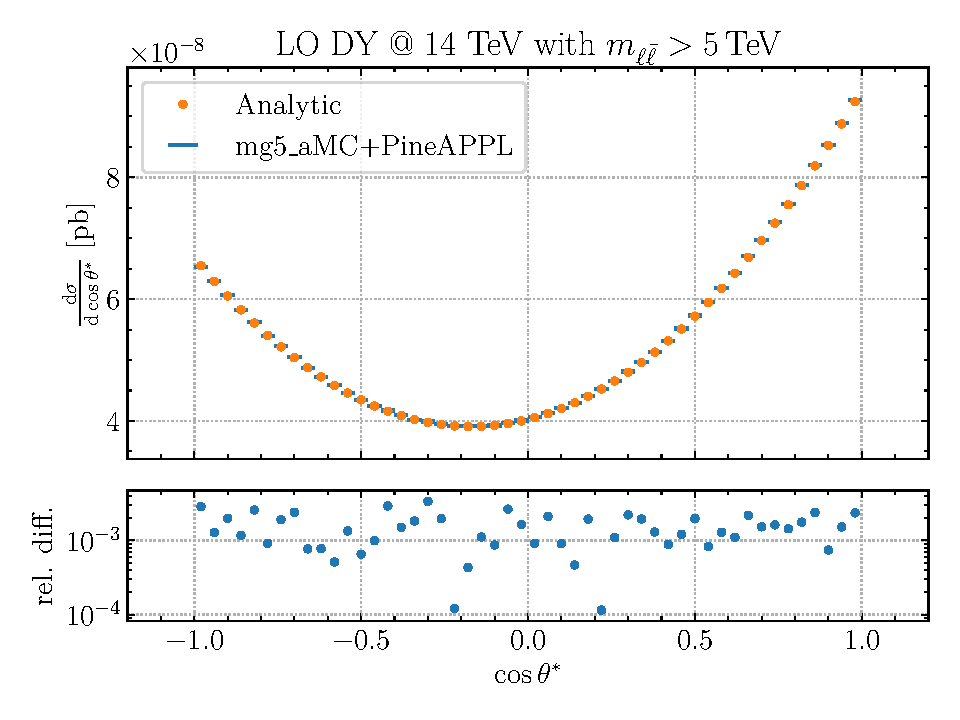
\includegraphics[width=0.49\linewidth]{ch-afb/sigma_grid_ana-MLL_5000_COSTH-r3.pdf}
  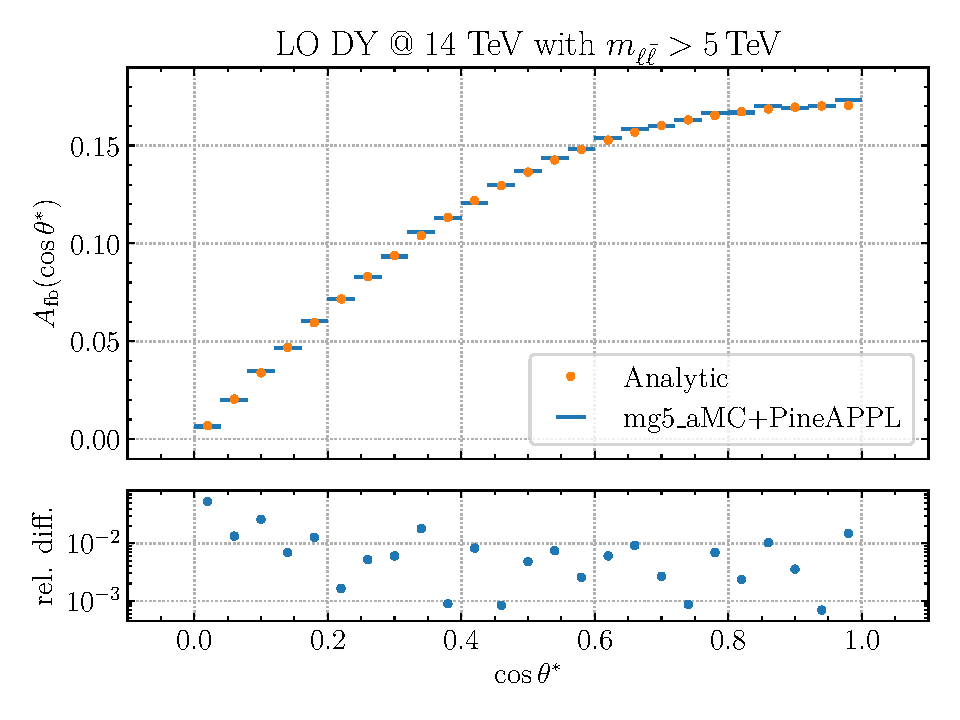
\includegraphics[width=0.49\linewidth]{ch-afb/afb_grid_ana-MLL_5000_COSTH-r3.pdf}
  \caption{The single-inclusive differential distribution in
    the Collins-Soper angle $\cos\theta^*$,
    \cref{eq:dsigma-dcos},
    and the corresponding forward-backward asymmetry computed at \lo,
    where the analytic calculation  \cref{eq:forward-backward-asymmetry}
    is compared with the numerical simulation based on 
    \mgamc
    interfaced to \pineappl.
    %
    The bottom panels display the relative difference between the analytic and
    numerical calculations.
    %
    One of the replicas of the \nnpdfr{4.0} \nnlo \pdf set is used as input
    to the calculation.
  }    
  \label{fig:lo-diff-cos}
\end{figure}
%%%%%%%%%%%%%%%%%%%%%%%%%%%%%%%

In order to illustrate concretely these results,  
in \cref{fig:lo-diff-cos} we display the
single-inclusive differential distribution in $\cos\theta^*$,
\cref{eq:dsigma-dcos},
and the corresponding forward-backward asymmetry,
\cref{eq:forward-backward-asymmetry} evaluated at \lo
for $\mll^{\text{min}}=\SI{5}{\TeV}$. The single-differential rapidity
distribution \cref{eq:dsigma-dyll}) is also shown for reference in \cref{fig:lo-diff-yll}.
%
We display both a numerical evaluation based on \mgamc interfaced to \pineappl,
as well as analytic results found using the form \cref{eq:lo-triple-diff-lumis}
of the triple differential luminosity, with all the values of the parameters
entering \crefrange{eq:coup}{eq:propzz} set to the values used in the \mgamc
runcard, and performing  numerically the integrals in
\cref{eq:dsigma-dcos,eq:dsigma-dyll}.
%
For validation purposes, no kinematic cuts are applied to the rapidities and
transverse momenta of final-state leptons.
The \pdf input is taken to be given, for illustrative purposes, by one of the
replicas of the \nnpdfr{4.0} \nnlo set.
The relative difference between the analytic and numerical calculation is shown
in the bottom panels of \cref{fig:lo-diff-cos} and demonstrates perfect
agreement. 

While the discussion so far has been presented  at \lo, its qualitative
features are unaffected by  higher-order corrections.
%
To illustrate this, in \cref{fig:lo-kfact} we compare the \lo result  from
\cref{fig:lo-diff-cos} to the corresponding \nlo \qcd result.
%
The bottom panels display the \nlo $K$-factor for the $\cos\theta^*$
distribution and the forward-backward asymmetry.
%
Whereas the \nlo $K$-factor in the $\cos\theta^*$ distribution is quite large
(around 40\%) it exhibits only a mild dependence on the Collins-Soper angle.
%
For $A_{\text{fb}}$, the $K$-factor is at the 10\% level and essentially
independent of the value of $\cos\theta^*$.

%%%%%%%%%%%%%%%%%%%%%%%%%%%%%%%%%%%%
\begin{figure}[t]
  \centering
  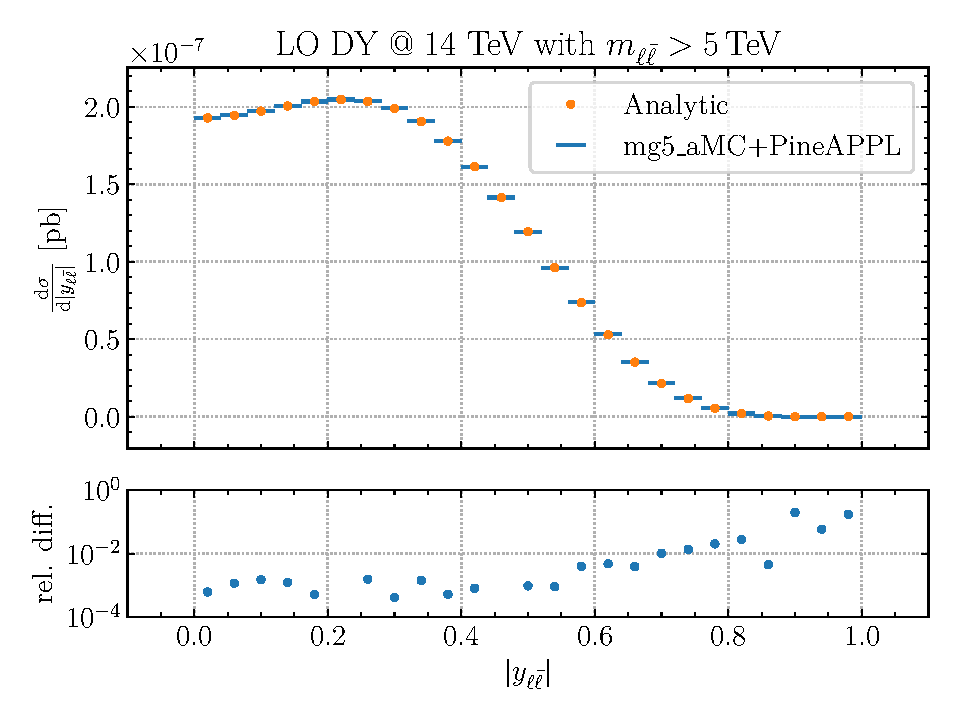
\includegraphics[width=0.49\linewidth]{ch-afb/sigma_grid_ana-MLL_5000_YLL-r3.pdf}
  \caption{Same as \cref{fig:lo-diff-cos} but now for the absolute dilepton rapidity distribution $|\yll|$}
  \label{fig:lo-diff-yll}
\end{figure}
%%%%%%%%%%%%%%%%%%%%%%%%%%%%%%%%%%%%%%%%%%
 
%%%%%%%%%%%%%%%%%%%%%%%%%%
\begin{figure}[t]
  \centering
  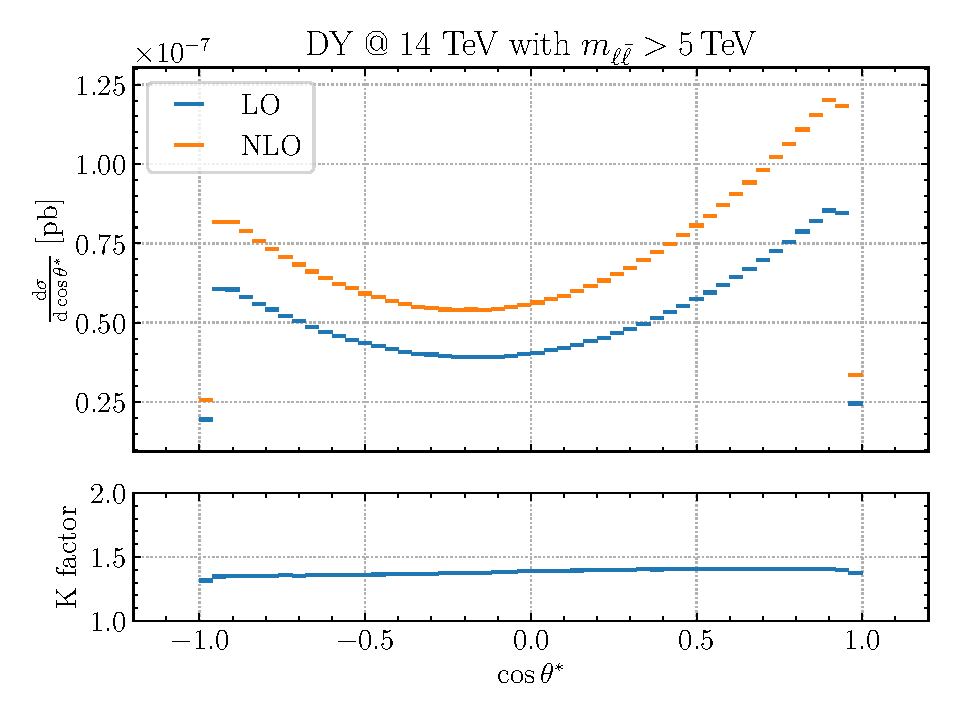
\includegraphics[width=0.49\linewidth]{ch-afb/sigma_lo_nlo-MLL_5000_COSTH-r3.pdf}
  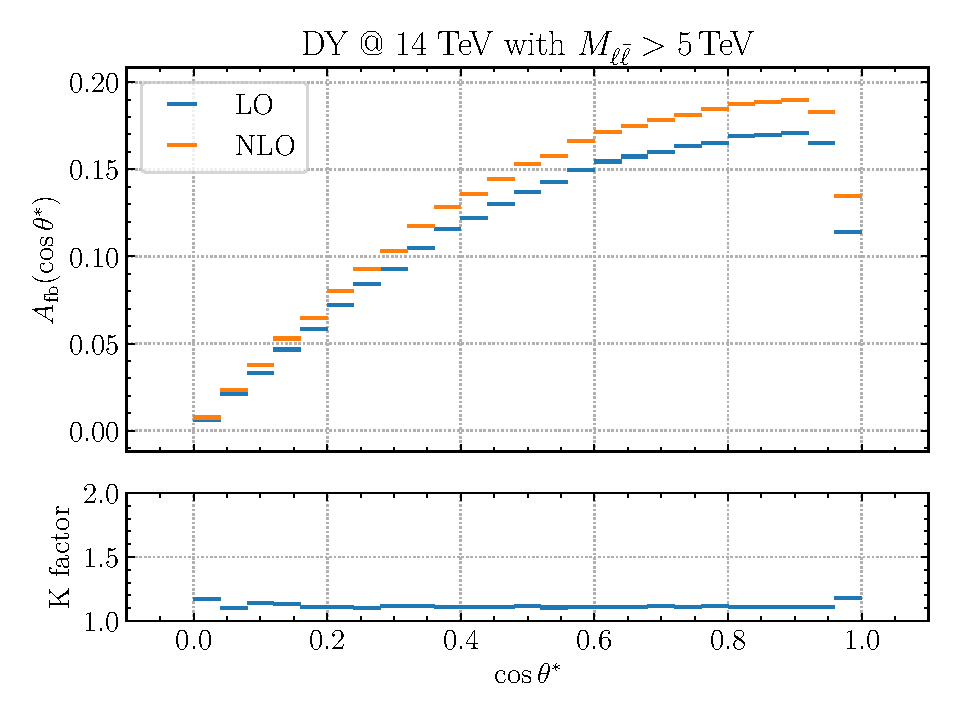
\includegraphics[width=0.49\linewidth]{ch-afb/afb_lo_nlo-MLL_5000_COSTH-r3.pdf}
  \caption{Same as \cref{fig:lo-diff-cos} now comparing the \lo result
    to the \nlo \qcd result obtained using \mgamc.
    %
    The $K$-factor is shown in the lower panel.
  }
  \label{fig:lo-kfact}
\end{figure}
%%%%%%%%%%%%%%%%%%%%%%%%%
